\documentclass[aspectratio=169,11pt]{beamer}

\usetheme{Madrid}
\usecolortheme{default}
\setbeamertemplate{navigation symbols}{}
\setbeamertemplate{footline}[frame number]

\usepackage{booktabs}
\usepackage{graphicx}
\usepackage{amsmath}
\usepackage{xcolor}

\definecolor{improve}{RGB}{44, 160, 44}
\definecolor{worsen}{RGB}{214, 39, 40}

\title{Polynomial Hint Preconditioning\\for Universal Time Series Forecasting}
\subtitle{Key Findings Summary}
\date{March 2026}

\begin{document}

% ============================================================
\begin{frame}
\titlepage
\end{frame}

% ============================================================
\begin{frame}{The Problem: Cross-Patch Information Bottleneck}

\textbf{Moirai-2}: Patch-based transformer for universal time series forecasting.

\medskip

\begin{columns}
\begin{column}{0.55\textwidth}
\begin{itemize}
    \item Input split into non-overlapping patches of 16 time steps
    \item Each patch embedding is \textbf{blind} to neighboring patches before attention
    \item Cross-patch patterns (daily cycles, weekly trends) must be discovered entirely by self-attention
\end{itemize}
\end{column}
\begin{column}{0.42\textwidth}
\centering
\fbox{\parbox{0.9\textwidth}{\centering
\textbf{Our fix:} Concatenate a polynomial-filtered channel\\[0.4em]
$\tilde{h}[t] = T_4(B^{16})\, x[t] - x[t]$\\[0.2em]
{\small $= -2\,x[t{-}32] + 0.5\,x[t{-}64]$}\\[0.4em]
{\small Injects info from patches $i{-}2$, $i{-}4$}\\[0.3em]
\textbf{+12K params (0.11\%)}\\
\textbf{+1.6\% compute}
}}
\end{column}
\end{columns}

\end{frame}

% ============================================================
\begin{frame}{Main Result: Capacity-Controlled Comparison (5 Seeds, 97 Configs)}

\begin{table}
\centering
\footnotesize
\begin{tabular}{lcccc}
\toprule
\textbf{Method} & \textbf{Mean MASE} & \textbf{Std} & \textbf{Wins / 485} & \textbf{$p$-value} \\
\midrule
\textcolor{improve}{\textbf{HD10 (Chebyshev hint)}} & \textcolor{improve}{\textbf{1.1765}} & 0.012 & \textcolor{improve}{\textbf{329 (67.8\%)}} & $\mathbf{1.5 \times 10^{-15}}$ \\
Zero channel & 1.2061 & 0.014 & 262 (54.0\%) & 0.042 \\
Baseline (no hint) & 1.2116 & 0.009 & --- & --- \\
\textcolor{worsen}{Duplicate channel} & \textcolor{worsen}{1.2162} & 0.011 & \textcolor{worsen}{217 (44.7\%)} & 0.99 \\
\bottomrule
\end{tabular}
\end{table}

\medskip

\begin{center}
\textbf{Duplicate HURTS} $\rightarrow$ not extra capacity \qquad
\textbf{Zero is neutral} $\rightarrow$ not wider projection

\medskip
\textcolor{improve}{\textbf{HD10 wins massively $\rightarrow$ polynomial content is what matters}}
\end{center}

\end{frame}

% ============================================================
\begin{frame}{Per-Seed Robustness}

\begin{table}
\centering
\footnotesize
\begin{tabular}{ccccc}
\toprule
\textbf{Seed} & \textbf{Baseline} & \textbf{HD10 (Ours)} & \textbf{Zero} & \textbf{Duplicate} \\
\midrule
0 & 1.2185 & \textcolor{improve}{\textbf{1.1577}} & 1.2072 & 1.2341 \\
1 & 1.1955 & \textcolor{improve}{\textbf{1.1902}} & 1.2285 & 1.2016 \\
2 & 1.2134 & \textcolor{improve}{\textbf{1.1798}} & 1.1845 & 1.2179 \\
7 & 1.2198 & \textcolor{improve}{\textbf{1.1698}} & 1.2053 & 1.2094 \\
42 & 1.2111 & \textcolor{improve}{\textbf{1.1852}} & 1.2048 & 1.2177 \\
\midrule
\textbf{Mean} & 1.2116 & \textcolor{improve}{\textbf{1.1765}} & 1.2061 & 1.2162 \\
\textbf{Std} & 0.009 & 0.012 & 0.014 & 0.011 \\
\bottomrule
\end{tabular}
\end{table}

\medskip
\centering
HD10 wins \textbf{every single seed}. Seed-averaged: \textbf{72/97 configs improve} ($p < 10^{-6}$).

\end{frame}

% ============================================================
\begin{frame}{Learning Rate Interaction}

\begin{table}
\centering
\footnotesize
\begin{tabular}{lccc}
\toprule
& $\eta = 10^{-3}$ & $\eta = 2 \times 10^{-3}$ & LR sensitivity \\
\midrule
Baseline & 1.2116 & 1.1841 & \textcolor{worsen}{2.27\%} \\
HD10 & 1.1765 & 1.1755 & \textcolor{improve}{0.09\%} \\
\midrule
HD10 vs BL & $-2.89\%$ \ \ ($p < 10^{-15}$) & $-0.72\%$ \ \ ($p = 3.8 \times 10^{-4}$) & \\
\bottomrule
\end{tabular}
\end{table}

\medskip

\begin{itemize}
    \item At matched LR: HD10 still wins (\textbf{280/485, $p=0.00038$}), but smaller effect
    \item HD10 is \textbf{LR-robust}: same performance at $10^{-3}$ and $2\times10^{-3}$
    \item Baseline is \textbf{LR-sensitive}: 2.27\% gap
    \item \textbf{Two benefits}: optimization robustness ($\sim$2.2\%) + genuine inductive bias ($\sim$0.7\%)
\end{itemize}

\end{frame}

% ============================================================
\begin{frame}{Where Does It Help?}

\begin{columns}
\begin{column}{0.48\textwidth}
\centering
\textbf{By Domain} {\footnotesize(5 seeds pooled)}\\[0.3em]
\footnotesize
\begin{tabular}{lrl}
\toprule
Domain & $\Delta$\% & Sig \\
\midrule
Demographics & +9.8\% & ** \\
Transport & +6.9\% & *** \\
Energy & +4.0\% & *** \\
M4 Comp. & +3.8\% & ** \\
IT/Cloud & +2.2\% & *** \\
ETT & +1.5\% & ** \\
Retail & +0.9\% & ns \\
\textcolor{gray}{Weather} & \textcolor{gray}{+0.3\%} & \textcolor{gray}{ns} \\
\textcolor{gray}{Healthcare} & \textcolor{gray}{+0.2\%} & \textcolor{gray}{ns} \\
\bottomrule
\end{tabular}
\end{column}
\begin{column}{0.48\textwidth}
\centering
\textbf{By Frequency}\\[0.3em]
\footnotesize
\begin{tabular}{lrl}
\toprule
Frequency & $\Delta$\% & Sig \\
\midrule
Sub-hourly & +3.4\% & *** \\
Hourly & +3.8\% & *** \\
Daily & +0.8\% & * \\
Weekly & +0.7\% & ** \\
Monthly & +3.4\% & ns \\
Quarterly & +0.2\% & ns \\
Yearly & +5.9\% & ns \\
\bottomrule
\end{tabular}

\bigskip

{\footnotesize Strongest at sub-hourly/hourly\\where filter lookback aligns\\with diurnal patterns}
\end{column}
\end{columns}

\end{frame}

% ============================================================
\begin{frame}{Per-Configuration Waterfall (5-Seed Average)}

\begin{center}
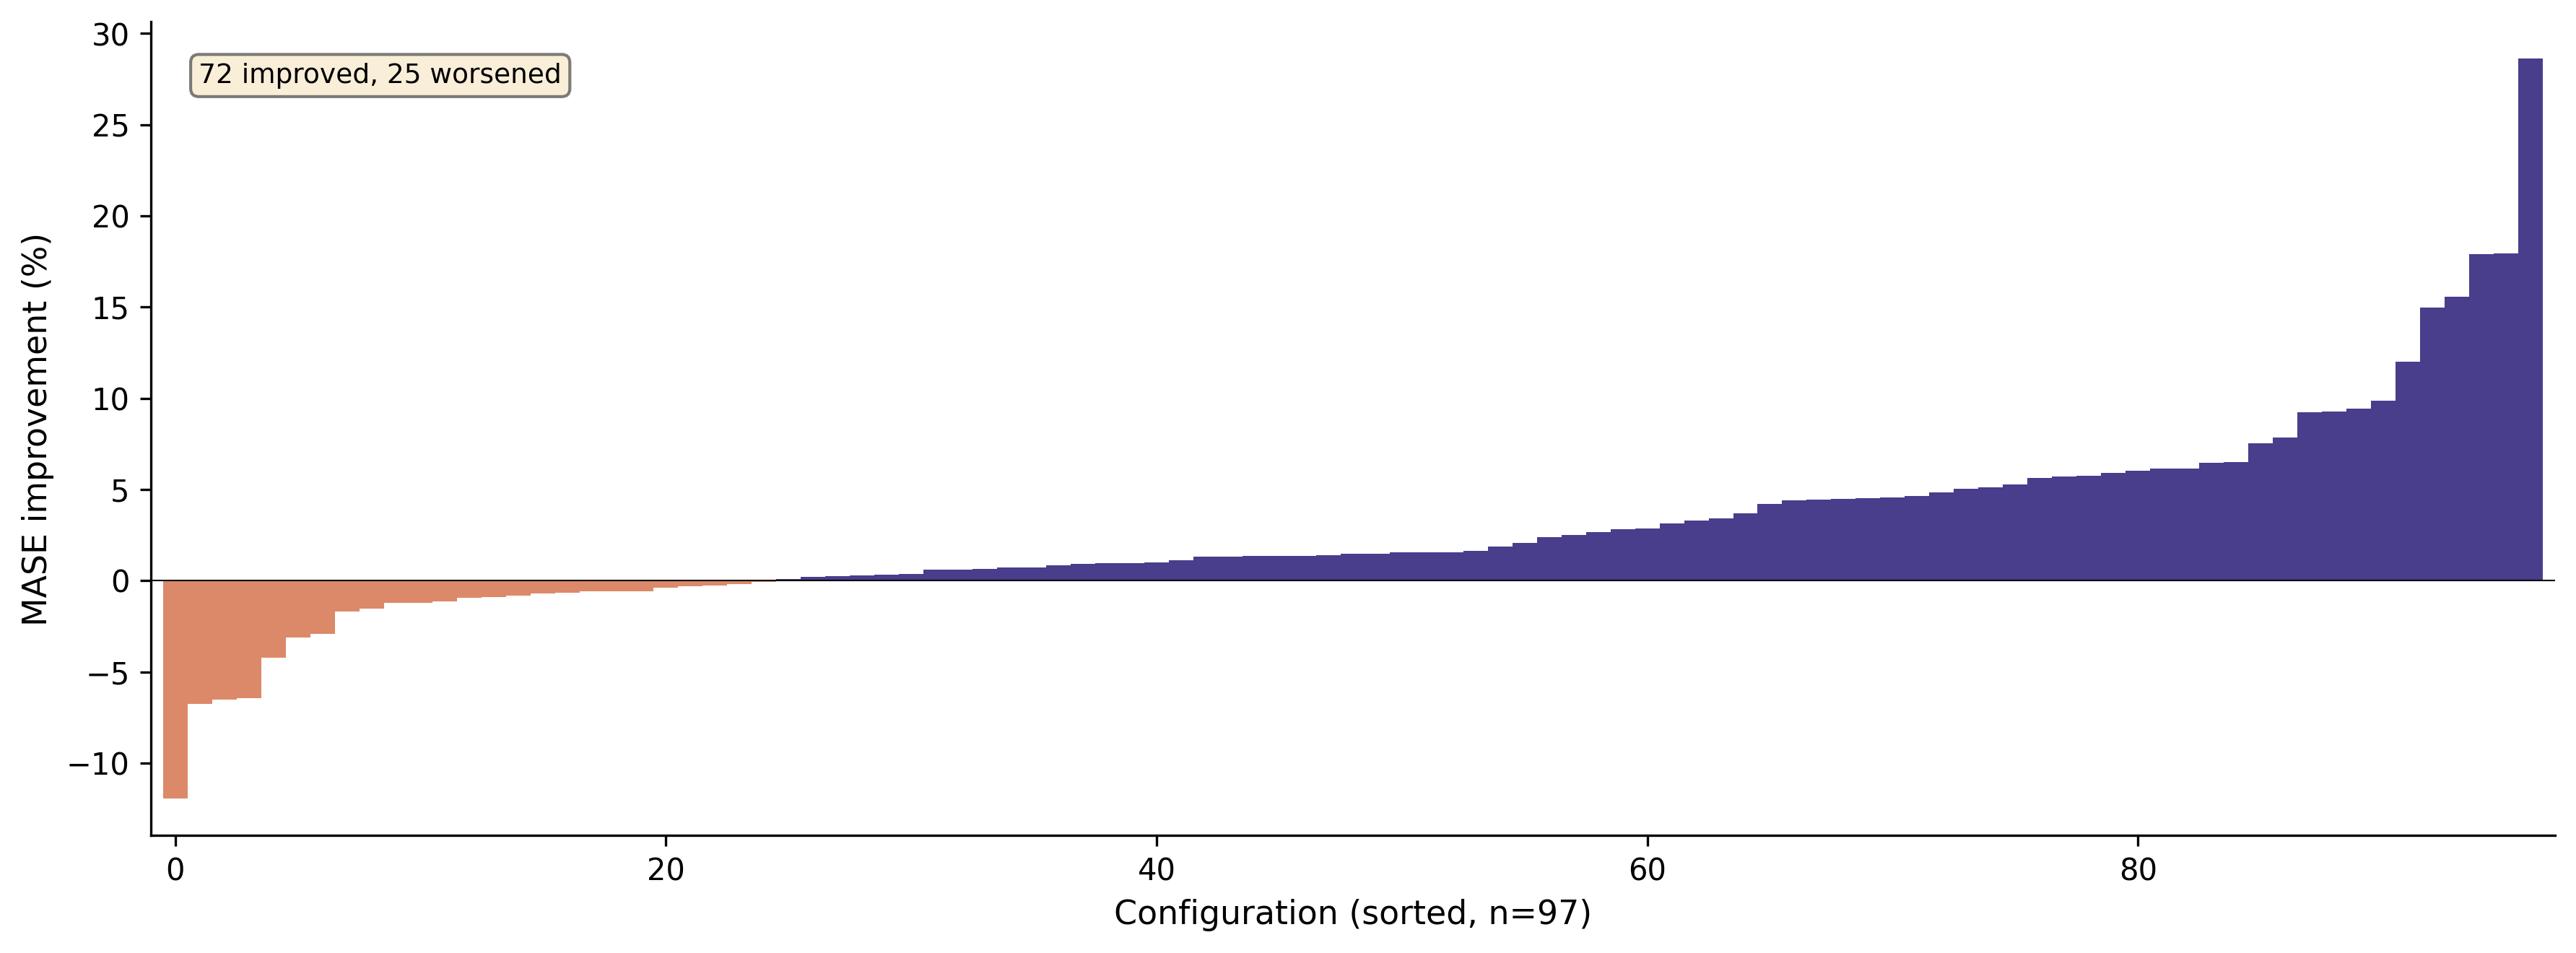
\includegraphics[width=0.82\linewidth]{figures/fig_waterfall.pdf}
\end{center}

\vspace{-0.5em}
{\small\textbf{72/97 configs improve}. Best: traffic (+18\%), solar long (+29\%). Worst: weekly ETT ($-12\%$), short solar ($-7\%).}

\end{frame}

% ============================================================
\begin{frame}{Ablations: Degree, Stride, Filter Basis, Dropout}

\begin{center}
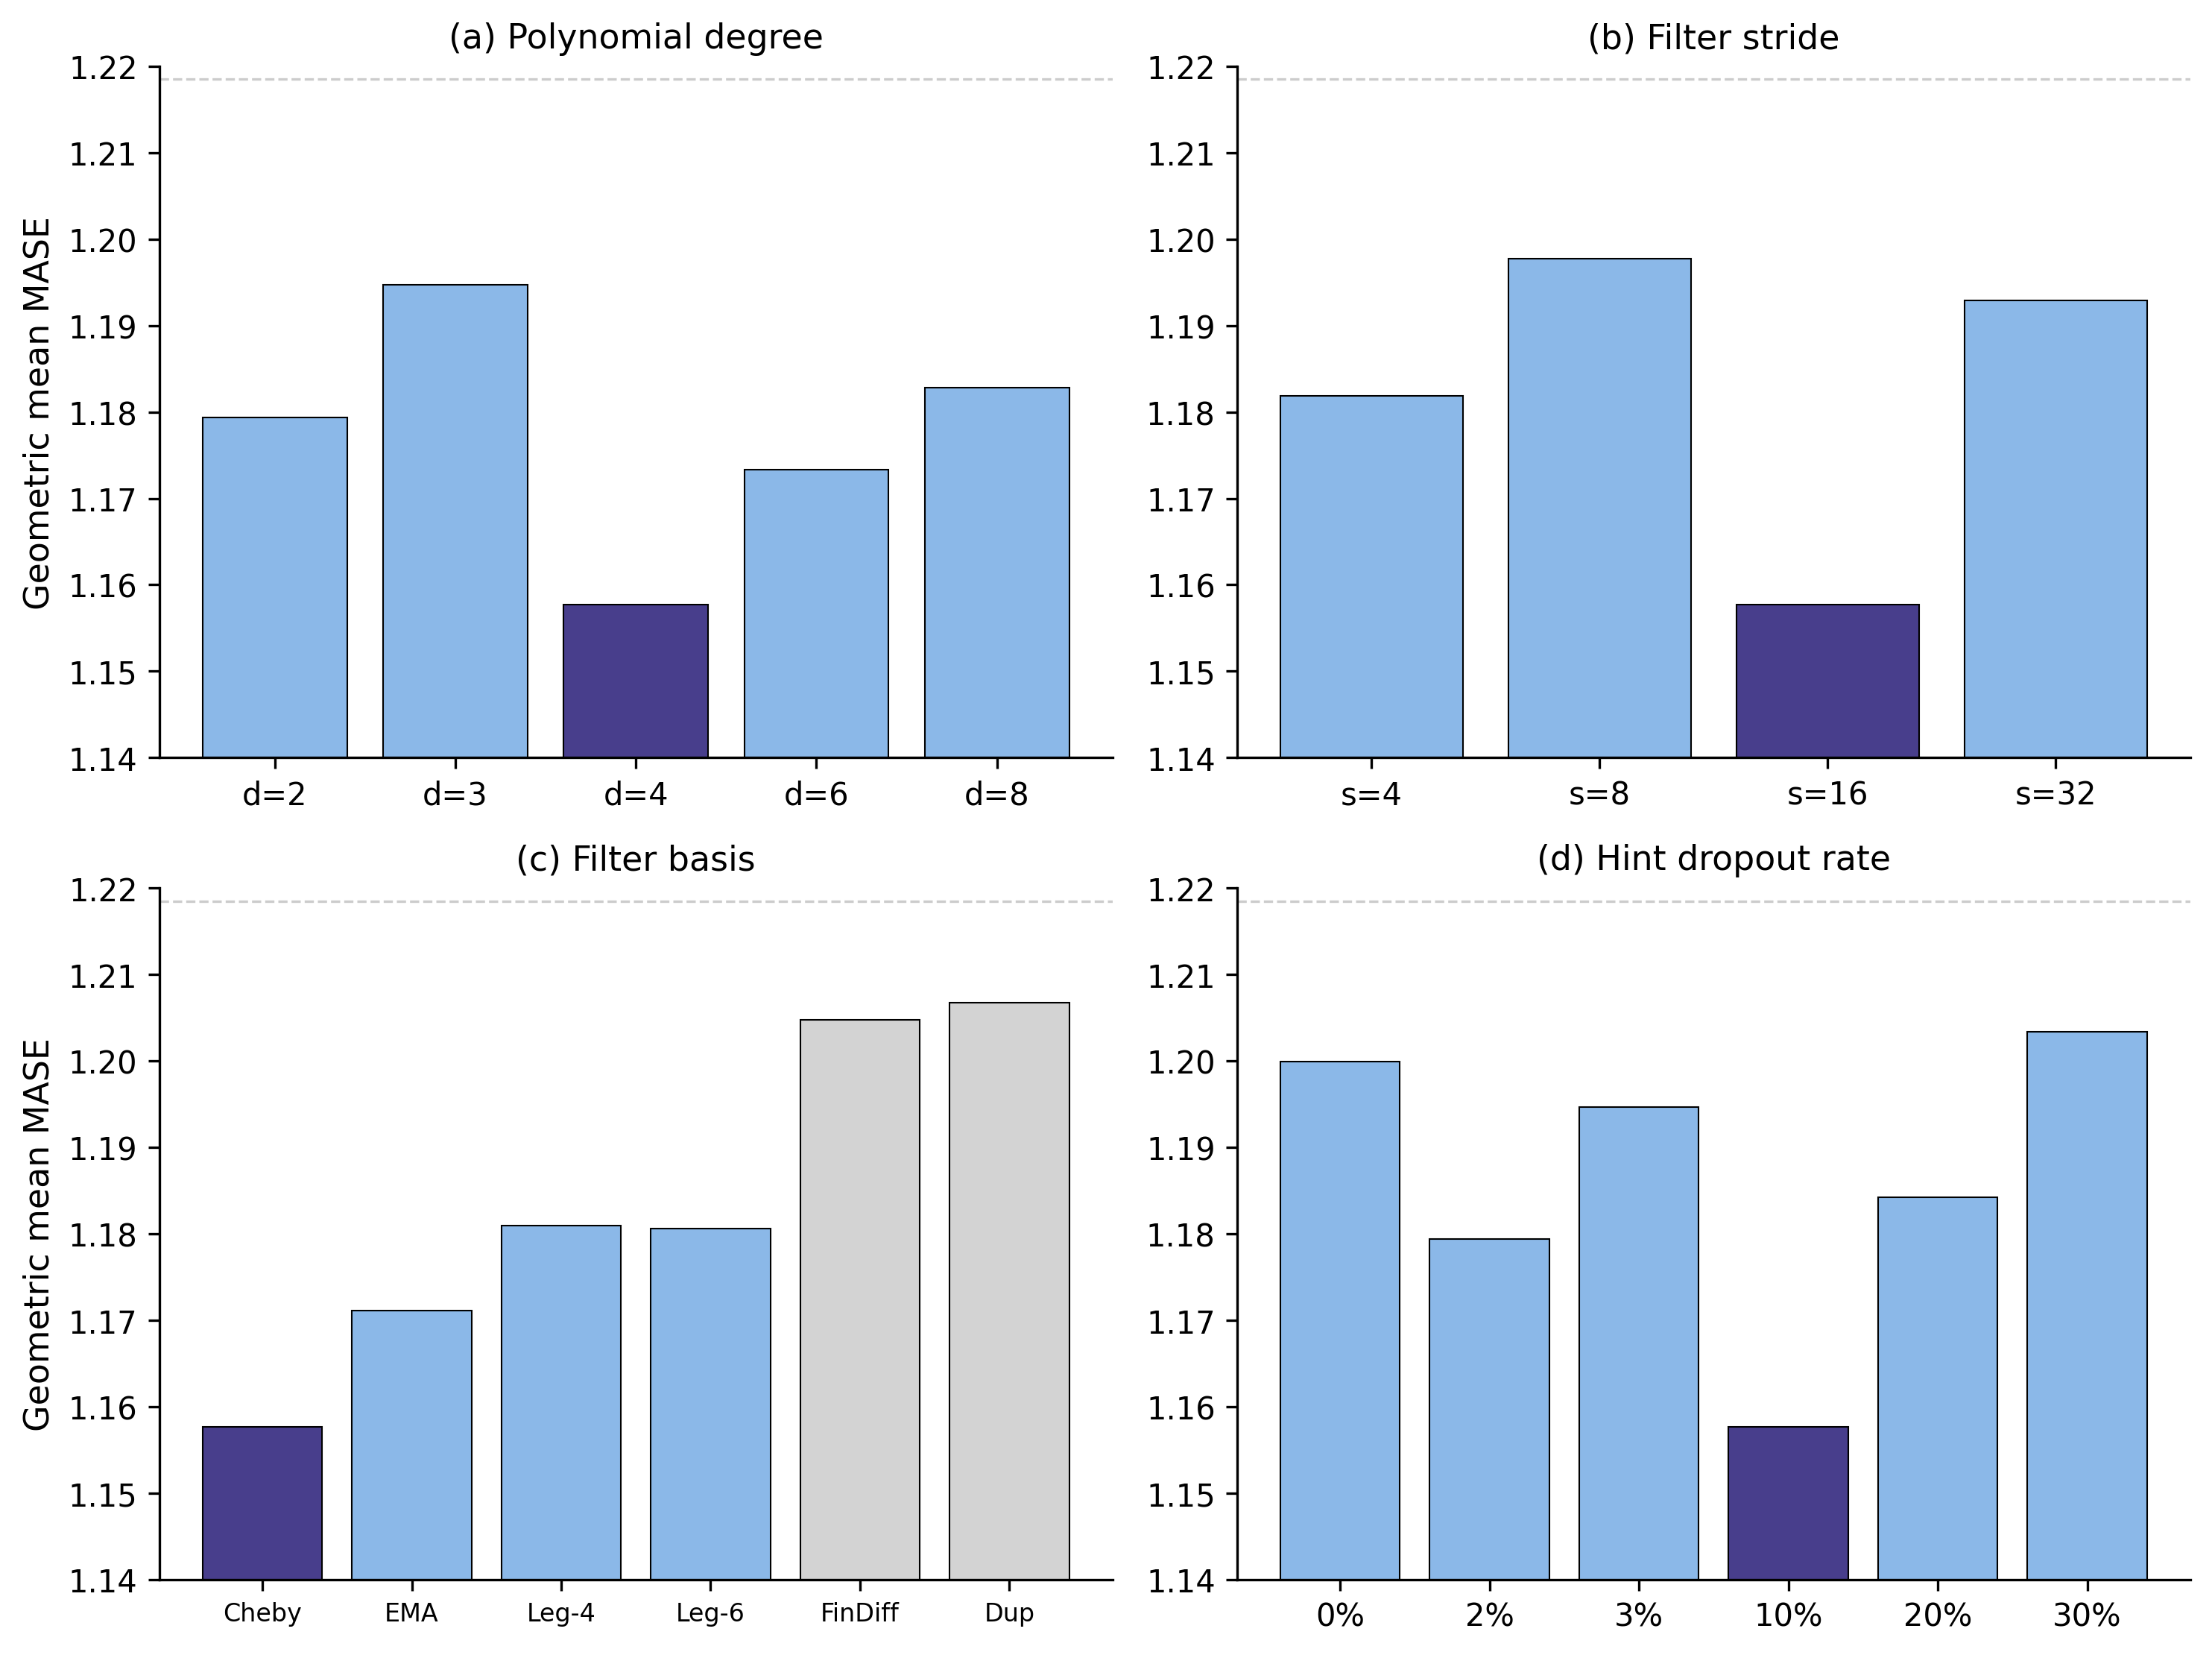
\includegraphics[width=0.78\linewidth,height=0.72\textheight,keepaspectratio]{figures/fig2_ablations.pdf}
\end{center}

\vspace{-0.5em}
{\small \textbf{Optimal}: Chebyshev degree 4, stride = patch size (16), 10\% hint dropout.}

\end{frame}

% ============================================================
\begin{frame}{The Model Learns Polynomial Structure}

\textbf{Train} with Chebyshev hints, then \textbf{evaluate} with different hint content:

\medskip

\begin{table}
\centering
\footnotesize
\begin{tabular}{lcc}
\toprule
\textbf{Hint at inference} & \textbf{MASE} & \textbf{vs Normal} \\
\midrule
\textcolor{improve}{Normal (Chebyshev)} & \textcolor{improve}{1.1577} & --- \\
No hint (baseline architecture) & 1.2185 & +5.2\% \\
Zeros & 1.2658 & +9.3\% \\
Random Gaussian noise & 1.3254 & +14.5\% \\
\textcolor{worsen}{Duplicate (copy of input)} & \textcolor{worsen}{1.5043} & \textcolor{worsen}{+29.9\%} \\
\bottomrule
\end{tabular}
\end{table}

\medskip
\centering
Random/duplicate hints are \textbf{worse than no hint at all}.\\
The model has learned to exploit the \textbf{specific polynomial structure}.

\end{frame}

% ============================================================
\begin{frame}{100K Training (Full Moirai-2 Budget, 3 Seeds)}

\begin{table}
\centering
\footnotesize
\begin{tabular}{lcccc}
\toprule
& Seed 0 & Seed 2 & Seed 7 & Mean \\
\midrule
Baseline & 1.2783 & 1.2138 & 1.2149 & 1.2357 \\
HD10 & 1.1739 & 1.2072 & 1.1880 & \textcolor{improve}{\textbf{1.1897 ($-3.7\%$)}} \\
MSHD10 & 1.1622 & 1.1856 & 1.1862 & \textcolor{improve}{\textbf{1.1780 ($-4.7\%$)}} \\
\bottomrule
\end{tabular}
\end{table}

\medskip

\begin{itemize}
    \item HD10 beats BL on all 3 seeds at full 100K training budget
    \item BL seed 0 collapses at 80K steps (cosine LR $\rightarrow$ 0); seeds 2, 7 don't
    \item \textbf{Pending}: 100K capacity controls (Dup/Zero) and LR schedule controls
\end{itemize}

\end{frame}

% ============================================================
\begin{frame}{Summary}

\begin{columns}
\begin{column}{0.55\textwidth}
\begin{enumerate}
    \item \textbf{Polynomial hints work}: $-2.89\%$ MASE, 329/485 wins, $p = 10^{-15}$
    \item \textbf{Not capacity}: duplicate hurts, zero neutral
    \item \textbf{LR-robust}: HD10 invariant to LR; BL sensitive
    \item \textbf{Matched LR}: $+0.72\%$, $p=0.0004$
    \item \textbf{Best config}: Cheby $d{=}4$, $s{=}P$, 10\% dropout
    \item \textbf{Best for}: high-freq, long horizon
    \item \textbf{Cost}: 0.11\% params, 1.6\% compute
\end{enumerate}
\end{column}
\begin{column}{0.42\textwidth}
\centering
\textbf{Pending experiments:}\\[0.5em]
\footnotesize
\begin{itemize}
    \item HD0 (0\% dropout, 5 seeds)
    \item Dup/Zero at LR=2e-3
    \item Dup/Zero at 100K
    \item LR schedule controls
    \item Official Moirai-2 calibration
\end{itemize}
\end{column}
\end{columns}

\end{frame}

\end{document}
